\capitulo{5}{Aspectos relevantes del desarrollo del proyecto}

En este apartado se recogen los detalles con mayor importancia en el desarrollo del proyecto. Tratando de mantener un orden cronológico con el que se puede observar los pasos que hemos seguido para solucionar las problemáticas del trabajo.

\begin{comment}
Este apartado pretende recoger los aspectos más interesantes del desarrollo del proyecto, comentados por los autores del mismo.
Debe incluir desde la exposición del ciclo de vida utilizado, hasta los detalles de mayor relevancia de las fases de análisis, diseño e implementación.
Se busca que no sea una mera operación de copiar y pegar diagramas y extractos del código fuente, sino que realmente se justifiquen los caminos de solución que se han tomado, especialmente aquellos que no sean triviales.
Puede ser el lugar más adecuado para documentar los aspectos más interesantes del diseño y de la implementación, con un mayor hincapié en aspectos tales como el tipo de arquitectura elegido, los índices de las tablas de la base de datos, normalización y desnormalización, distribución en ficheros3, reglas de negocio dentro de las bases de datos (EDVHV GH GDWRV DFWLYDV), aspectos de desarrollo relacionados con el WWW...
Este apartado, debe convertirse en el resumen de la experiencia práctica del proyecto, y por sí mismo justifica que la memoria se convierta en un documento útil, fuente de referencia para los autores, los tutores y futuros alumnos.
\end{comment}

\section{Procesamiento de imágenes}
\label{procimg}
Como primera aproximación al problema que nos concierne, nos hemos enfrentado al procesamiento de imágenes mediante la librería \textit{Scikit-image} de \textit{Python}. Mediante esta herramienta trataremos de dar solución a nuestro problema siguiendo los siguientes pasos:

\begin{enumerate}[1.]
  \item Convertir la imagen a escala de grises
  \item Segmentar los objetos del fondo de la imagen
  \item Obtener los distintos objetos de la imagen
\end{enumerate}

\subsection{Convertir la imagen a escala de grises}

La conversión de la imagen original (RGB) a escala de grises viene motivada por el hecho de que los fitolitos carecen de color, por lo que es información que no nos interesa, y con el objetivo de poder segmentar los objetos del fondo de la imagen mediante el método de \textit{Thresholding}. Solo pudiéndose partir de una imagen en escala de grises. En la figura \ref{fig:5.1.1} podemos ver los resultados.

\begin{figure}
	\centering
	\begin{subfigure}[b]{0.45\textwidth}
        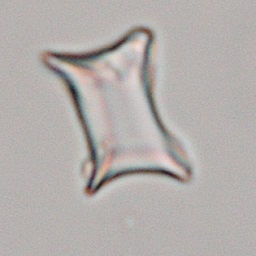
\includegraphics[width=\textwidth]{2}
        \caption{Original}
    \end{subfigure}
    \hspace{1em}
    \begin{subfigure}[b]{0.45\textwidth}
        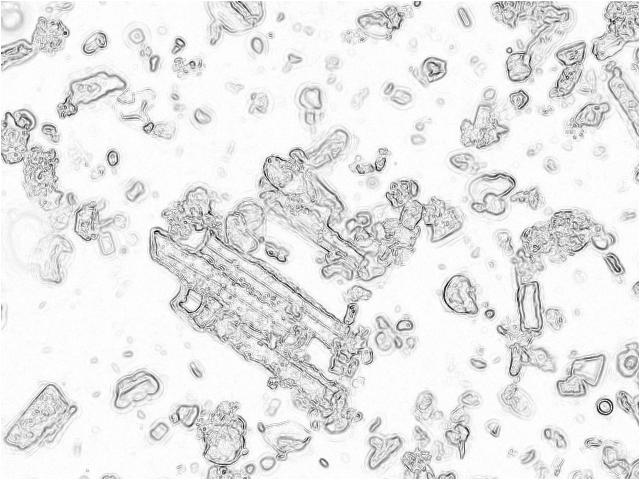
\includegraphics[width=\textwidth]{grayscale_image}
        \caption{Imagen en escala de grises}
    \end{subfigure}
    \caption{Conversión de la imagen original a escala de grises}
	\label{fig:5.1.1}
\end{figure}

\subsection{Segmentar los objetos del fondo de la imagen}

Una vez tenemos la imagen en escala de grises, procedemos a transformarla en una imagen en blanco y negro o binarizada. Los motivos por los que binarizamos la imagen es para obtener una imagen que sea más significativa para nosotros y además este simplificada. Lo cual nos será útil para facilitarnos su procesamiento.

\textit{Scikit-image} nos propociona distintos métodos mediante los cuales podemos segmentar una imagen. En la figura \ref{fig:5.1.2} podemos observar el resultado aplicando distintos métodos, los cuales se van indicando en cada una de las figuras.

\begin{figure}
	\centering
	\begin{subfigure}[b]{0.45\textwidth}
        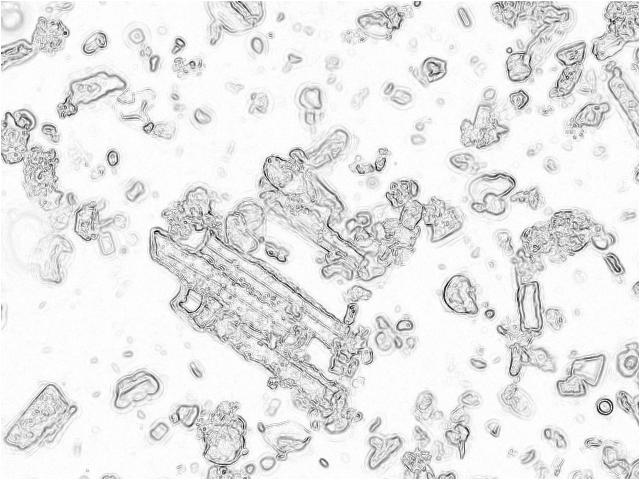
\includegraphics[width=\textwidth]{grayscale_image}
        \caption{Imagen en escala de grises}
    \end{subfigure}
    \begin{subfigure}[b]{0.45\textwidth}
        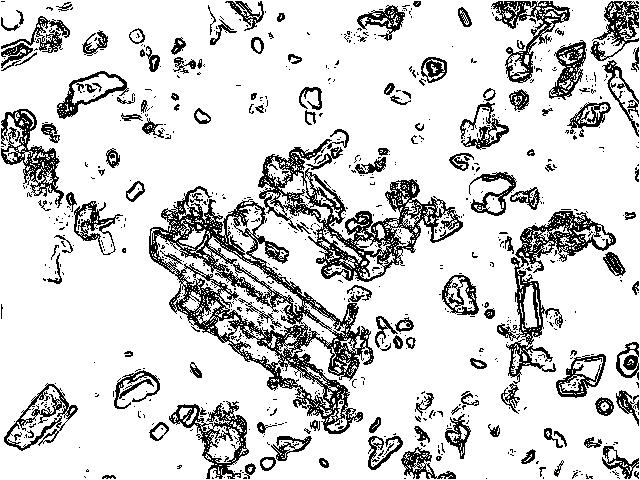
\includegraphics[width=\textwidth]{otsu_threshold_image}
        \caption{Método de Otsu}
    \end{subfigure}
    \begin{subfigure}[b]{0.45\textwidth}
        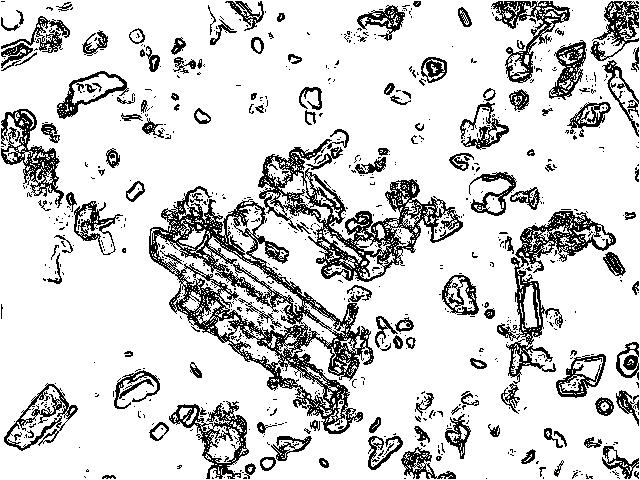
\includegraphics[width=\textwidth]{otsu_threshold_image}
        \caption{Método de Otsu}
    \end{subfigure}
    \begin{subfigure}[b]{0.45\textwidth}
        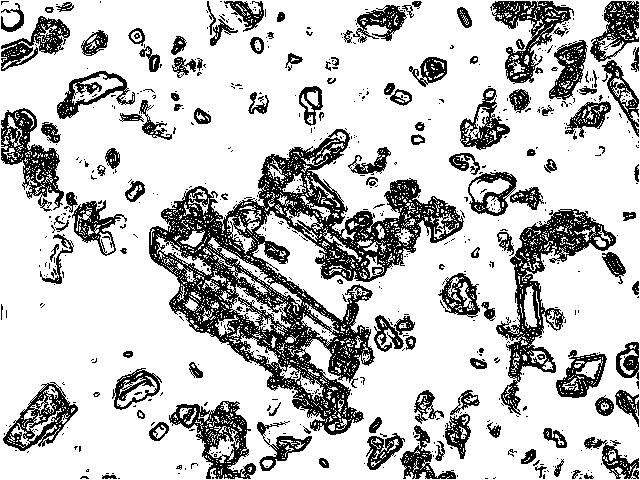
\includegraphics[width=\textwidth]{yen_image}
        \caption{Método de Yen}
    \end{subfigure}
    \begin{subfigure}[b]{0.45\textwidth}
        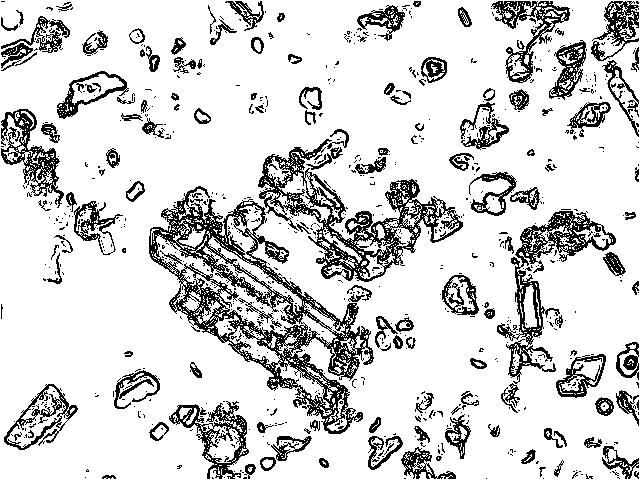
\includegraphics[width=\textwidth]{li_thresholded_image}
        \caption{Método de Li}
    \end{subfigure}
    \begin{subfigure}[b]{0.45\textwidth}
        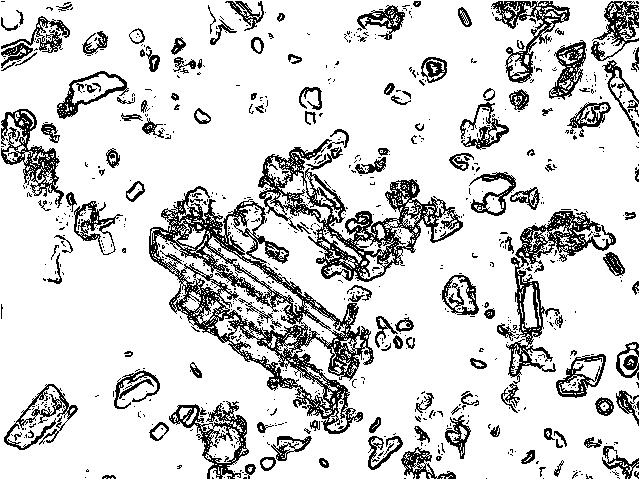
\includegraphics[width=\textwidth]{isodata_thresholded_image}
        \caption{Método de ISODATA}    
    \end{subfigure}
    \begin{subfigure}[b]{0.45\textwidth}
        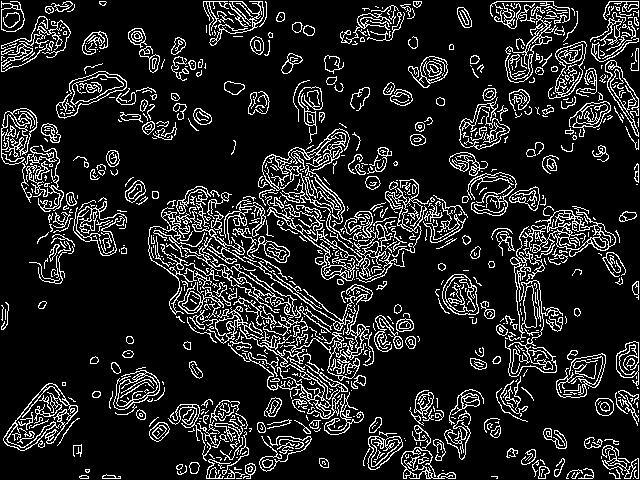
\includegraphics[width=\textwidth]{edge_based_image}
        \caption{Método basado en bordes}    
    \end{subfigure}
    \begin{subfigure}[b]{0.45\textwidth}
        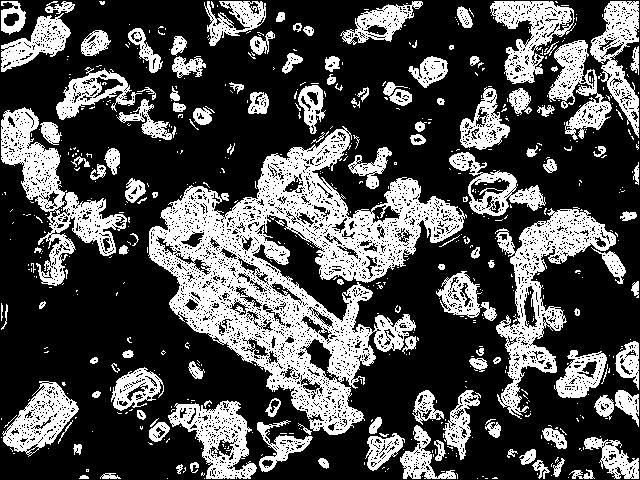
\includegraphics[width=\textwidth]{adaptive_thresholded_image_5}
        \caption{Método adaptativo}    
    \end{subfigure}
    \caption{Distintos ejemplos de una imagen segmentada}
	\label{fig:5.1.2}
\end{figure} 

\subsection{Obtener los distintos objetos de la imagen}
Después de tener la imagen binarizada de la forma más apropiada posible probamos a segmentar los distintos objetos de nuestra imagen.

\subsection{Transformación divisoria}
Transformación divisoria, o en inglés \textit{Watershed segmentation}, es un algoritmo clásico para la segmentación de objetos en una imagen~\cite{wiki:watershed}.

Durante las primeras pruebas, la segmentación más interesante hasta el momento ha sido la que se muestra en la figura \ref{fig:5.1.3}. A partir de \textit{Watershed segmentation} con marcado, representando cada color un objeto distinto. Más allá de esta segmentación no se ha conseguido nada mejor.

\begin{figure}
	\centering
	\begin{subfigure}[b]{0.45\textwidth}
        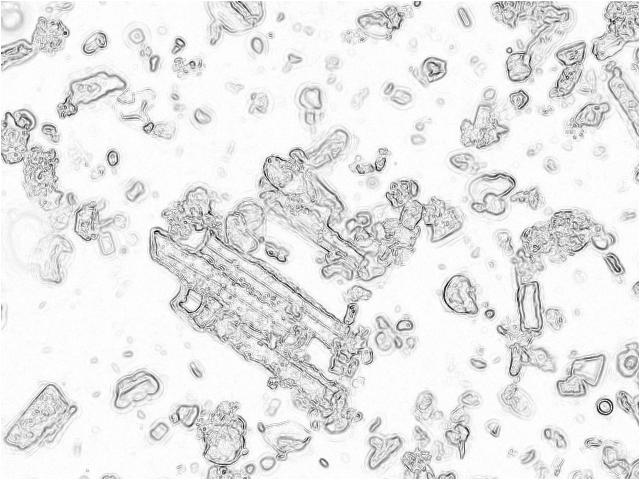
\includegraphics[width=\textwidth]{grayscale_image}
        \caption{Imagen en escala de grises}
    \end{subfigure}
    \begin{subfigure}[b]{0.45\textwidth}
        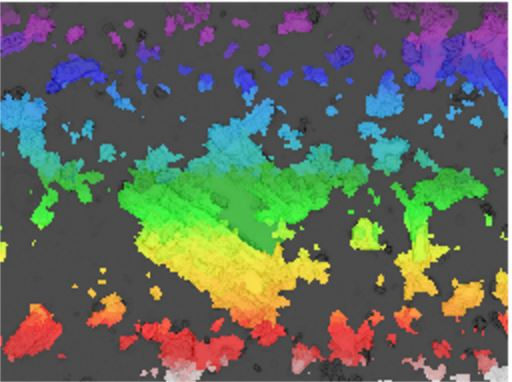
\includegraphics[width=\textwidth]{segmented}
        \caption{Imagen segmentada}
    \end{subfigure}
        \caption{Resultados obtenidos mediante transformación divisoria}
	\label{fig:5.1.3}
\end{figure} 	

\section{Problema fundamental: falta de imágenes}

Llegados a este punto, y teniendo una primera aproximación, con mayor o menor precisión, de como afrontar el reconocimiento automático de fitolitos, se plantea un problema fundamental en el desarrollo de este proyecto. El problema al que me refiero, es que no poseemos o conocemos ningún conjunto de entrenamiento de imágenes etiquetadas\footnote{Me refiero por imágenes etiquetadas, a imágenes con las coordenadas de donden se encuentran los distintos fitolitos en estas.} de fitolitos. Y por lo que consideramos, es el requisito básico en el aprendizaje supervisado.

Debido a esta problemática, desarrollamos un etiquetador de fitolitos que permita a nuestros usuarios crear un conjunto de imágenes de fitolitos etiquetadas y así, solucionar este problema fundamental en el desarrollo del proyecto.

En concreto, este etiquetador es una aplicación web desarrollada sobre un conjunto de tecnologías \textit{Python} y \textit{JavaScript}. Con el objetivo de poder realizar un futuro despliegue en un servicio \textit{web} que facilite lo máximo las tareas a nuestros usuarios. Aunque en su desarrollo resultó en un problema, por la falta de manuales que enseñasen como llevarlo a cabo y la complejidad que introduce la comunicación entre \textit{Python} y \textit{JavaScript}. La información más detallada para un futuro programador, o para el uso por parte del usuario, se encuentra en los anexos del manual del programador y el manual del usuario, respectivamente.

\section{Clasificadores}

La aproximación mediante procesamiento de imágenes, mostrada previamente en la sección \ref{procimg}, no parece la más adecuada visto los resultados obtenidos. Por ello vamos a realizar el estudio sobre una segunda aproximación  mediante clasificadores, junto a descriptores visuales y la técnica de la ventana deslizante, o en inglés \textit{sliding window}.

\textit{Sliding window} consiste en la subdivisión de una imagen en distintos fragmentos, estableciendo previamente el tamaño de los fragmentos, tanto en ancho como en alto, y el tamaño del salto en cada eje, tras una subdivisión. 

Como podemos apreciar en la figura \ref{fig:sliding_window}, primero la ventana deslizante recorre la imagen en el eje horizontal. Comenzando por la esquina superior izquierda hasta llegar a la esquina superior derecha. Generando una imagen por cada subdivisión y realizando saltos horizontales según el tamaño que hayamos definido. Una vez esta llega a la esquina superior derecha, la ventana deslizante lleva a cabo el mismo proceso pero realizando un salto en el eje vertical. Y así sucesivamente hasta completar su recorrido por toda la imagen.

\begin{figure}
\centering
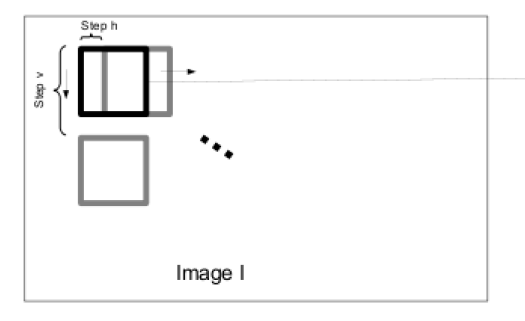
\includegraphics[width=0.8\textwidth]{sliding_window}
\caption[Esquema del funcionamiento de la ventana deslizante]{Esquema del funcionamiento de la ventana deslizante~\cite{jcp}}
\label{fig:sliding_window}
\end{figure}

Después de completar el recorrido, cada uno de los recortes resultantes se envía a un clasificador, el cual distingue a que clase pertenece el recorte. Por ejemplo, fitolito o no fitolito (fondo de la imagen).

El primer conjunto de técnicas escogidas ha sido una Máquina de Vector Soporte (SVM)~\cite{svm} junto al Histograma de los gradientes orientados, la cual es una técnica para la extracción automática de características. Sin embargo, se analizaron distintas técnicas para adoptar la que mejor se adapte a nuestra problemática.

El procedimiento para obtener el clasificador es el siguiente:

\begin{enumerate}[1.]
  \item Crear un conjunto de entrenamiento de imágenes de caras que consideramos que son elementos positivos.
  \item Crear un conjunto de entrenamiento de imágenes de no-caras que consideramos que son negativos.
  \item Extraer las características del conjunto de entrenamiento  mediante un descriptor visual.
  \item Entrenar\footnote{Nos referimos por entrenar, en este ámbito, a enviar al clasificador las distintas imágenes con la clase a la que pertenecen (fitolito de tipo 1, fitolito de tipos 2, etc.).} el clasificador.
\end{enumerate}

 Finalizado el entrenamiento, ya tenemos nuestro clasificador listo para enviarle nuevas imágenes y que sean clasificadas.
 
\subsection{Reconocimiento de imágenes en nuevas imágenes}
Para el reconocimiento de objetos en nuevas imágenes, deberemos llevar a cabo los tres siguientes pasos:

\begin{enumerate}[1.]
  \item Dividir la imagen en múltiples fragmentos.
  \item Comprobar si cada uno de los fragmentos contiene el objeto.
  \item Si existe solapamiento en la detección de objetos, muy común en el uso de este tipo de clasificadores, se deben de combinar dichos solapamientos en uno único.
\end{enumerate}

Cada uno de los fragmentos anteriores se solapa en gran medida. Por lo que origina un problema de sobrereconocimiento de objetos, reconociendo donde existe un posible positivo, más de uno, en la mayoría de casos. Por ello, se aplica el tercer paso sobre los objetos reconocidos, que es la eliminación del solapamiento de objetos mediante la técnica de \textit{Non-maximum suppression}.

\subsection{Aplicación sobre el reconocimiento de caras}

Como previa experimentación con esta metodología, vamos a entrenar el clasificador para el reconocimiento de caras. Y en función de la efectividad del método sobre las caras tomaremos una serie de conclusiones sobre las que decidiremos si llevar a cabo esta solución sobre  nuestro problema.

Como explicábamos anteriormente, una vez tenemos nuestro clasificador le enviamos una nueva imagen, como podría ser la presentada en la figura \ref{subfig:family}. A partir de esta imagen el clasificador nos permitirá obtener las ventanas \footnote{Se entiende por ventana, en este contexto, a la caja o cuadrilátero que etiqueta un positivo en una imagen.} en las que detecta una cara, como vemos en la figura \ref{subfig:family_labeled}. Podemos apreciar que existe más de una ventana alrededor de cada cara. Y finalmente, tras aplicar el método \textit{Non-Maximum supresion} obtenemos el resultado final mostrado en la figura \ref{subfig:family_labeled_nms}.

\begin{figure}
	\centering
	\begin{subfigure}[b]{0.45\textwidth}
        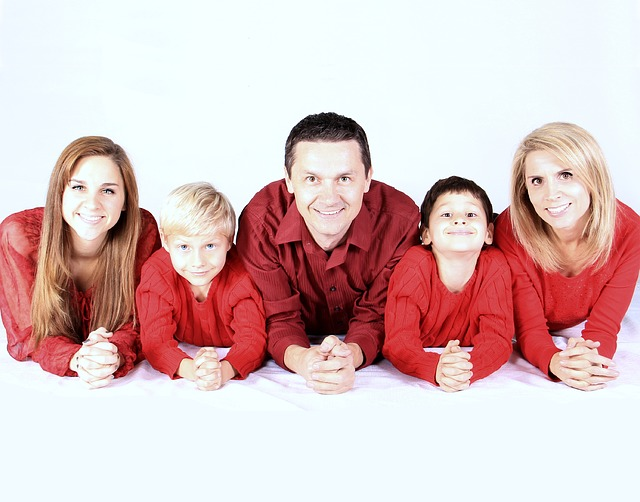
\includegraphics[width=\textwidth]{family}
        \caption{Imagen de la cual se desean identificar las caras}
        \label{subfig:family}
    \end{subfigure}
    \begin{subfigure}[b]{0.45\textwidth}
        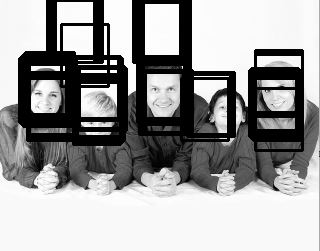
\includegraphics[width=\textwidth]{family_labeled}
        \caption{Imagen después de aplicarla nuestro clasificador}
        \label{subfig:family_labeled}
    \end{subfigure}
    \begin{subfigure}[b]{0.45\textwidth}
        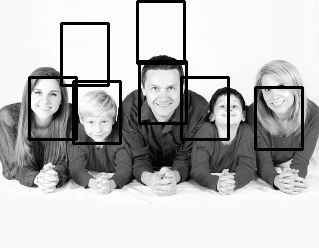
\includegraphics[width=\textwidth]{family_labeled_nms}
        \caption{Imagen tras aplicarla \textit{Non-Maximum supresion}}
         \label{subfig:family_labeled_nms}
    \end{subfigure}
        \caption[Resultados tras aplicar el clasificador sobre una imagen]{Resultados tras aplicar el clasificador sobre una imagen. Imagen obtenida de la página web \url{www.pexels.com}}
	\label{fig:5.1.4}
\end{figure}

\subsection{Conclusiones}

El método utilizado en esta sección se encuentra muy limitado por los siguientes aspectos:

\begin{itemize}
	\item Es una técnica que presenta problemas de rendimiento. Puesto que requiere de 2 o 3 segundos, como mínimo, para clasificar una nueva imagen.
	\item Es una técnica que no tiene en cuenta el contexto de la imagen para su clasificación. Sino, que solo tiene en cuenta cada uno de los fragmentos de la imagen de manera aislada al resto. Lo cual dificulta una adecuada precisión del clasificador.
	\item Comete muchos errores en la detección de falsos positivos. Como se puede observar en la figura \ref{subfig:family_labeled_nms}.
	\item El tamaño de la subdivisión de la imagen es constante. Por lo tanto, complica las posibilidades en la detección de distintos tamaños de fitolitos.
\end{itemize}

\section{Detección de objetos mediante técnicas de \textit{deep learning}}

Una vez observados los resultados mediante una técnica clásica, como es \textit{sliding window}, vamos a ir un paso más allá, con las técnicas de \textit{deep learning}. Las cuales son las que, con diferencia, mayor rendimiento aportan en la actualidad, como previamente he explicado en los conceptos teóricos.

Para ello, vamos a entrenar una implementación de \textit{YOLO} en \textit{Python}, llamada \textit{darkflow}~\cite{darkflow}, todavía en desarrollo, para tratar de llevar a cabo el detector automático de fitolitos. Aunque, existen otras alternativas que se podrían adoptar en un futuro de no conseguir los resultados esperados con esta implementación.

Previamente, en los conceptos teóricos, se ha explicado que este tipo de modelos también presentan algunas problemáticas, por el volumen de imágenes necesario y el tiempo necesario para ser entrenados, principalmente. Existen soluciones, como \textit{data augmentation}, trasferencia de conocimiento o partir de modelos previamente entrenados.

Tras experimentar con estas técnicas durante un periodo de más de un mes, no se han conseguido resultados. Lo que quiero decir con esto es que el modelo entrenado no es capaz de obtener cajas al predecir una nueva imagen. Y, por lo tanto, la precisión es de un 0\%. Existen dos principales razones por las que el modelo no es capaz de obtener resultados, bajo el conocimiento que he adquirido sobre este marco de trabajo:

\begin{itemize}
	\item El modelo no es capaz de converger en un número de iteraciones en torno a 1000 \textit{epochs}\footnote{\textit{Epoch}: es una pasada por todas las capas de la red neuronal en ambos sentidos.}. Lo cual son más de 50 horas de entrenamiento.
	\item El modelo necesita cambios en algunas parametrizaciones de la red neuronal respecto a las utilizadas por el modelo original.
\end{itemize}

Adicionalmente, por si fuese de interés, incluyo 2 hilos de \textit{GitHub} en los que sé mantuvo conversaciones con los desarrolladores del proyecto y otros colaboradores para la puesta a punto del sistema: \url{www.github.com/thtrieu/darkflow/issues/256} y \url{www.github.com/thtrieu/darkflow/issues/80}.

Por concluir, al necesitar mejores recursos para el entrenamiento de la red, mayores conocimientos sobre el funcionamiento del modelo y debido a la alta complejidad del problema se mantiene esta posible solución como una segunda vía para continuar estudiando en líneas futuras.

\section{Solución final: \textit{Bag of Words} junto  a \textit{ventana deslizante}}

Como hemos observado durante el transcurso de este capítulo, hemos tratado de recorrer la mayoría de los caminos en visión artificial para dar solución a este problema. Comenzando por lo más sencillo y finalizando con lo más complejo.

Llegados a este punto, hemos podido ver que la solución de este problema con aprendizaje profundo o \textit{deep learning} no es trivial. Y, por lo tanto, para llevarlo a cabo adecuadamente es necesario tener conocimientos avanzados en este campo. Y que al contrario, la utilización de un clasificador junto a descriptores de características tiene una puesta a punto mucho más transparente para el desarrollador, aunque su rendimiento sea sustancialmente peor que el de una red neuronal.

Sin embargo, existe una solución derivada del uso de clasificadores junto a la ventana deslizante que soluciona algunos de los problemas de esta: \textit{Bag of Words} junto a ventana deslizante. A los problemas a los que hago referencia son:

\begin{itemize}
	\item Detectar fitolitos de distintos tamaños.
	\item Mejorar la precisión en la detección.
\end{itemize}

En cuanto a la primera problemática, cuando utilizamos un descriptor de características sobre una ventana o recorte de la imagen, obtenemos un resultado cuyo tamaño es dependiente de las dimensiones de la ventana que estemos utilizando. Esta ventana será la que después enviemos a nuestro clasificador para obtener una predicción. Teniendo que ser la ventana y la entrada de nuestro clasificador siempre de las mismas dimensiones. Por lo tanto, esto nos condiciona a que la ventana debe ser siempre de un tamaño fijo, aunque los fitolitos no lo sean.

Sin embargo, la técnica \textit{Bag of Words} soluciona esta problemática. Debido a que el resultado del descriptor se agrupa, mediante \textit{clustering}, en un número fijo de características independiente del tamaño de la ventana. Mediante el cual se predice si una determinada ventana contiene un fitolito.

Por otro lado, aun no teniendo una base con la que contrastar la mejoría de la precisión respecto al uso de un clasificador junto a un descriptor de características. Esta técnica se ha utilizado comúnmente por reportar mejores resultados. 

A continuación, se explica como hemos llegado al mejor clasificador para llevar a cabo esta tarea y los resultados obtenidos en materia de validación cruzada y reconocimiento de fitolitos.

\subsection{Obtención del mejor clasificador}

Para conseguir la mayor precisión posible, el primer paso consiste en conseguir el clasificador que mejor se ajuste a este problema. Para llevar a cabo esta tarea fundamental se prueban 11 clasificadores distintos, realizando cambios en sus parámetros y finalmente validando sus resultados mediante validación cruzada\footnote{Consiste en la evaluación de los resultados haciendo subdivisiones aleatorias entre el conjunto de datos para la evaluación y el entrenamiento. De manera que se consigan unos resultados que se asemejen lo máximo a los que conseguiremos en la práctica.}. De manera que lleguemos a la configuración que mejor se ajuste a este problema.

Para comprobar cual es la mejor combinación de parámetros posible dado un clasificador se utiliza un método de \textit{scikit-learn} que asigna combinaciones aleatorias entre los valores dados. Pudiéndose utilizar alternativamente la búsqueda en malla con resultados similares pero con una lentitud mucho mayor\footnote{Búsqueda en malla:~\url{http://scikit-learn.org/stable/modules/generated/sklearn.model_selection.GridSearchCV.html} y búsqueda aleatoria:~\url{www.scikit-learn.org/stable/modules/generated/sklearn.model_selection.RandomizedSearchCV.html}.}.

\subsection{Resultados experimentales}

Antes de comenzar a analizar los resultados, en esta primera versión vamos a barajar dos posibilidades: clasificar si una región es fitolito o no, o clasificar si una región es uno de los distintos tipos de fitolito o no, diferenciándolos entre sí. 

Por otro lado, en este apartado vamos a analizar los resultados obtenidos en la evaluación de los distintos clasificadores y en el reconocimiento de fitolitos.

\subsubsection{Validación cruzada}

Como previamente comentábamos, para la obtención del mejor clasificador utilizamos la validación cruzada mediante la cual obtendremos la precisión de un modelo dadas distintas subdivisiones sobre el conjunto de datos. En la figura~\ref{fig:cross_val} muestro una gráfica de los mejores resultados en la clasificación binaria de fitolitos, es decir, fitolito o no fitolito. Como podemos apreciar, conseguimos tasas mayores del 90\% de clasificación, lo cual representa que el clasficador predice correctamente en más del 90\% de los casos lo que es un fitolito y lo que no lo es. Hay que destacar que el conjunto de entrenamiento de la clase fitolito y fondo esta compuesta por aproximadamente 200 imágenes en cada caso. 

\begin{figure}
\centering
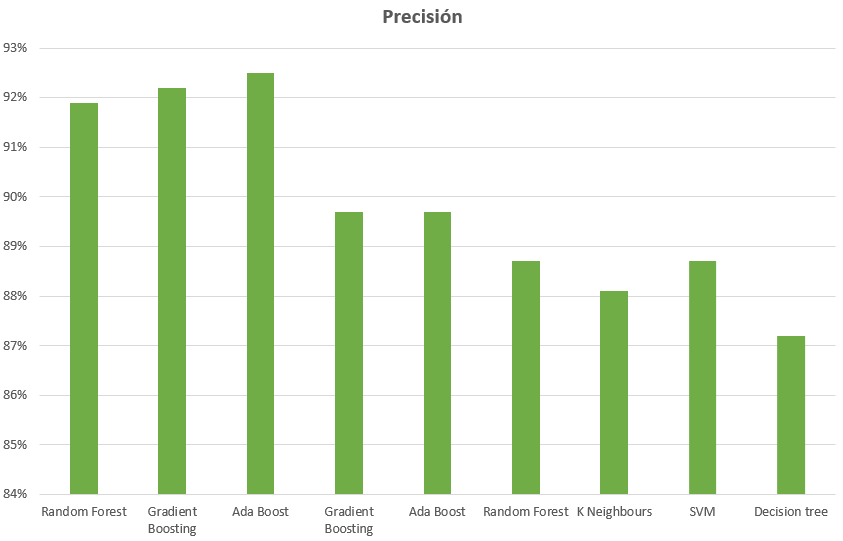
\includegraphics[width=1\textwidth]{cross_val}
\caption[Resultados de la validación cruzada con las clases fitolito y no fitolito]{Resultados de la validación cruzada con las clases fitolito y no fitolito. Algunos de los clasificadores se repiten por el hecho de que son resultados con distintos ajustes en los parámetros, tales como: el número de \textit{clusters} y clasificadores base, entre otros.}
\label{fig:cross_val}
\end{figure}

Por otro lado, se encuentra la clasificación en los distintos tipos de fitolitos. En este caso, debido a las restricciones de mis recursos \textit{hardware} solo puedo utilizar 50 imágenes por clase. Los mejores resultados como observamos en la gráfica~\ref{fig:cross_val_all} están en torno al 64\% de precisión. Lo cual nos lleva a la decisión final de que en esta primera versión solo tratemos de reconocer los fitolitos, sin categorizarles.

\begin{figure}
\centering
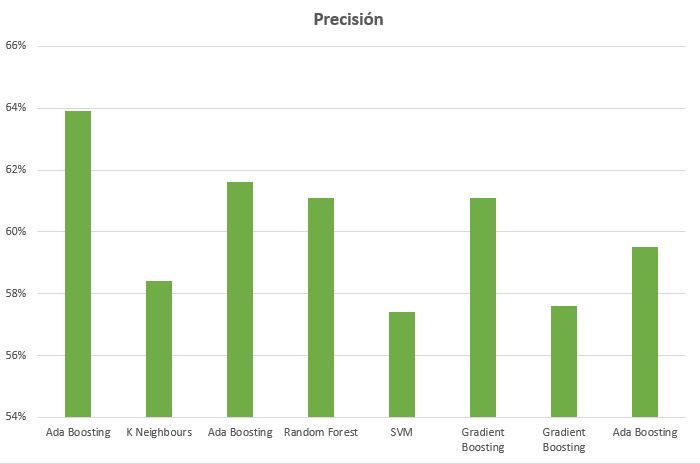
\includegraphics[width=1\textwidth]{cross_val_all_cls}
\caption{Resultados de la validación cruzada con los distintos tipos de fitolito}
\label{fig:cross_val_all}
\end{figure}

Para concluir, los resultados de la validación cruzada tienen el único objetivo de escoger el mejor modelo. A continuación, analizaremos los resultados del modelo aplicado al reconocimiento de fitolitos.

\subsubsection{Reconocimiento de fitolitos}

Para finalizar este trabajo, vamos a realizar un breve análisis de los resultados obtenidos sobre 10 imágenes escogidas aleatoriamente con las que nuestro clasificador no ha sido entrenado. En la figura~\ref{fig:5.17} muestro cuatro de ellas, tras predecirlas con nuestro sistema. Siendo las dos primeras muy pocos precisas y las dos últimas absolutamente precisas, pero con algo de imprecisión a la hora de delimitar al fitolito. Para no dejar lugar a la duda, en la figura~\ref{fig:5.18} muestro las imágenes orginales etiquetadas por nuestros colaboradores y expertos.

\begin{figure}
	\centering
	\begin{subfigure}[b]{0.45\textwidth}
        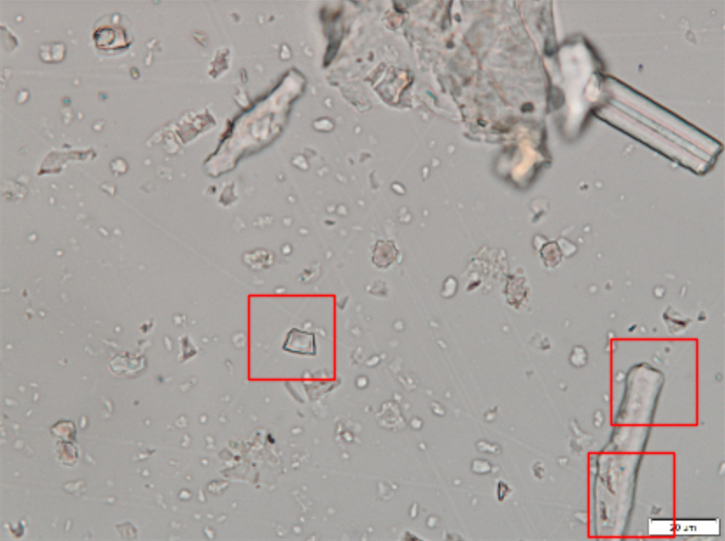
\includegraphics[width=\textwidth]{ex5}
        \caption{Ejemplo 1 predicho}
        \label{subfig:fej1}
    \end{subfigure}
    \begin{subfigure}[b]{0.45\textwidth}
        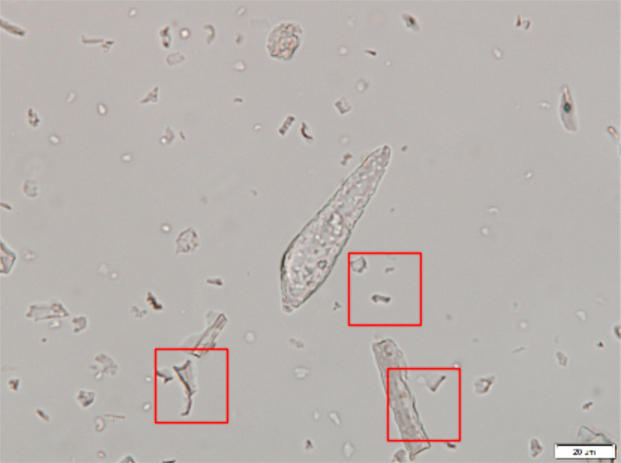
\includegraphics[width=\textwidth]{ex2}
        \caption{Ejemplo 2 predicho}
        \label{subfig:fej2}
    \end{subfigure}
    \begin{subfigure}[b]{0.45\textwidth}
        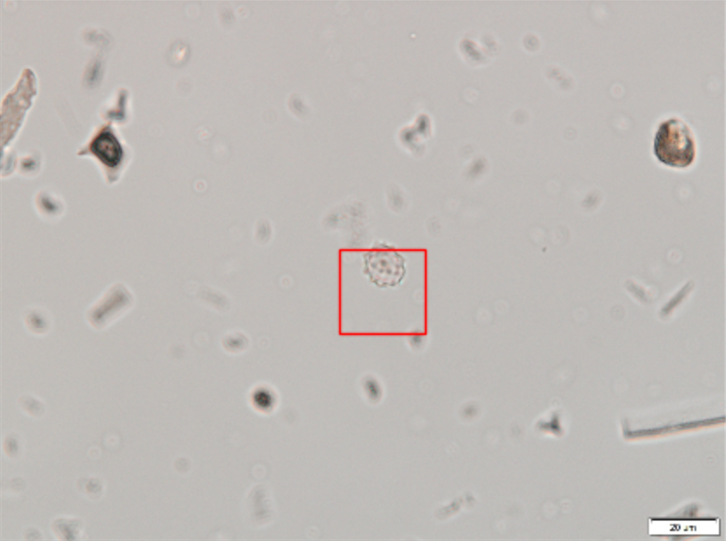
\includegraphics[width=\textwidth]{ex6}
        \caption{Ejemplo 3 predicho}
        \label{subfig:fe3}
    \end{subfigure}
    \begin{subfigure}[b]{0.45\textwidth}
        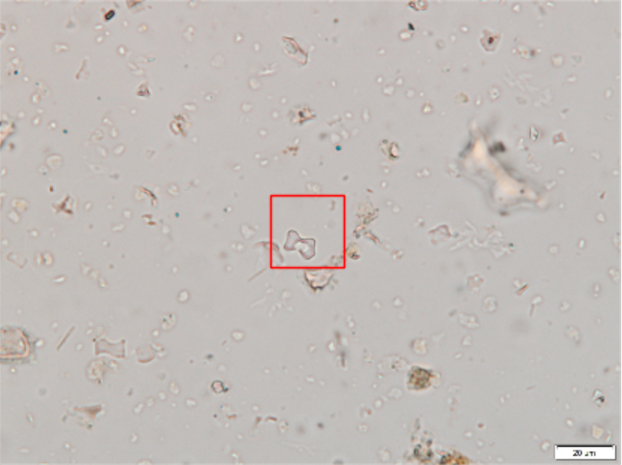
\includegraphics[width=\textwidth]{ex4}
        \caption{Ejemplo 4 predicho}
        \label{subfig:fe4}
    \end{subfigure}
        \caption{Resultados experimentales en el reconocimiento de fitolitos}
	\label{fig:5.17}
\end{figure}

\begin{figure}
	\centering
	\begin{subfigure}[b]{0.45\textwidth}
        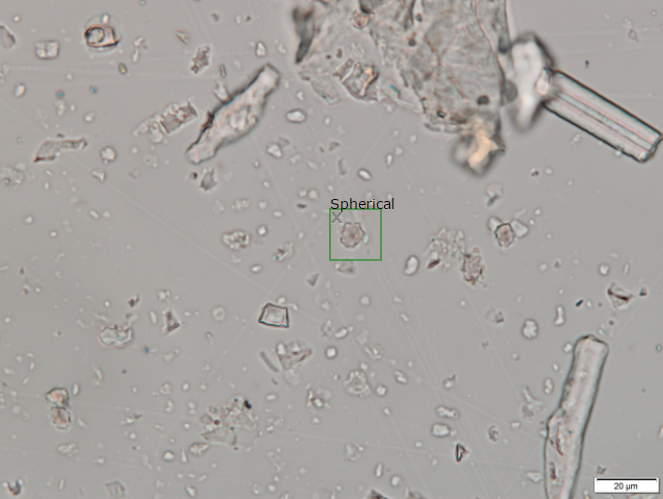
\includegraphics[width=\textwidth]{ex5c}
        \caption{Ejemplo 1}
        \label{subfig:fej1c}
    \end{subfigure}
    \begin{subfigure}[b]{0.45\textwidth}
        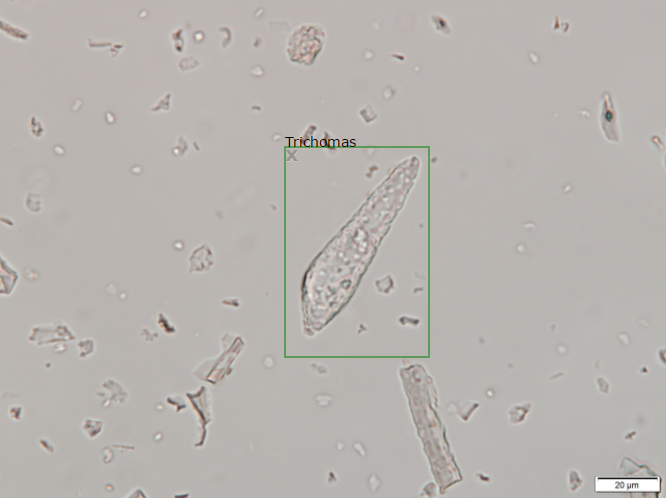
\includegraphics[width=\textwidth]{ex2c}
        \caption{Ejemplo 2}
        \label{subfig:fej2c}
    \end{subfigure}
    \begin{subfigure}[b]{0.45\textwidth}
        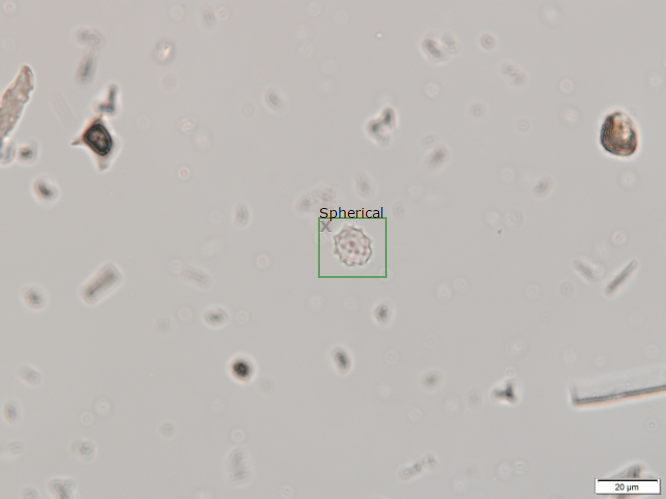
\includegraphics[width=\textwidth]{ex6c}
        \caption{Ejemplo 3}
        \label{subfig:fe3c}
    \end{subfigure}
    \begin{subfigure}[b]{0.45\textwidth}
        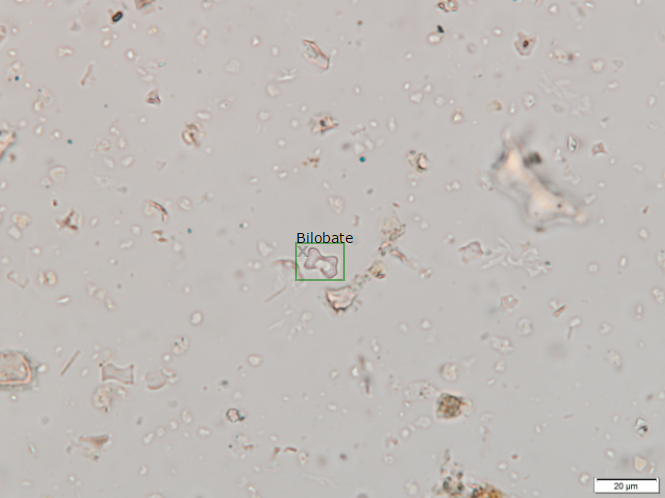
\includegraphics[width=\textwidth]{ex4c}
        \caption{Ejemplo 4}
        \label{subfig:fe4c}
    \end{subfigure}
        \caption{Imágenes originales}
	\label{fig:5.18}
\end{figure}

Para concluir, en la gráfica~\ref{fig:acc} muestro la precisión en el reconocimiento de fitolitos sobre las 10 imágenes con las que hemos evaluado a nuestro sistema. En esta muestro los verdaderos positivos por imagen, los falsos positivos y el total de fitolitos. Como se puede apreciar, en un 60\% de las imágenes se reconoce todos los fitolitos correctamente. Pero, sin embargo, en seis de las 10 imágenes se reconocen falsos positivos.

\begin{figure}
\centering
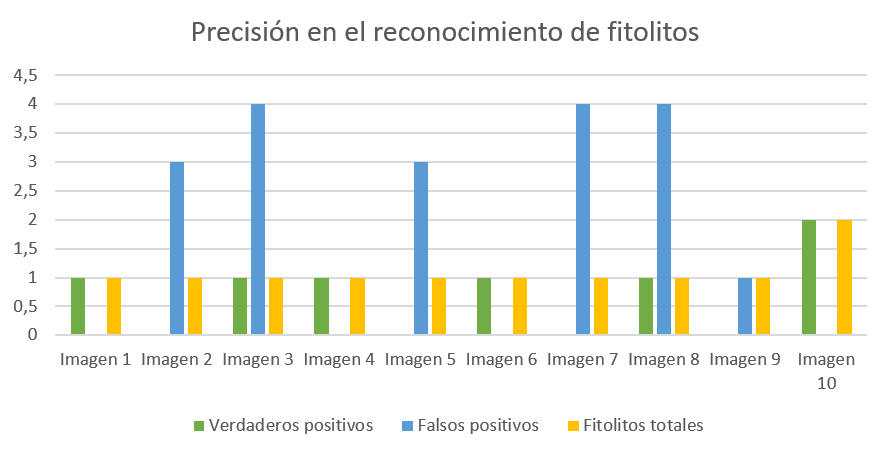
\includegraphics[width=1\textwidth]{acc}
\caption{Precisión en el reconocimiento de fitolitos}
\label{fig:acc}
\end{figure}